The requeriments of the water purification system are:

\begin{enumerate}

\item{} A high degree of purification of the water sample extracted from the dam, reducing its conductivity by approximately two orders of magnitude (from $1000~\mu$S$/\cm$ to $10~\mu$S$/\cm$).

\item{} Low maintenance cost  and manpower.

\item{} Software-based management of the system.
\end{enumerate}

The LARUEX laboratory in Extremadura, one of the six members of the TRITIUM collaboration, has designed, developed and built the water purification system, the scheme of which is shown in Figure \ref{fig:WPSScheme}.

\begin{figure}[htbp]
\centering
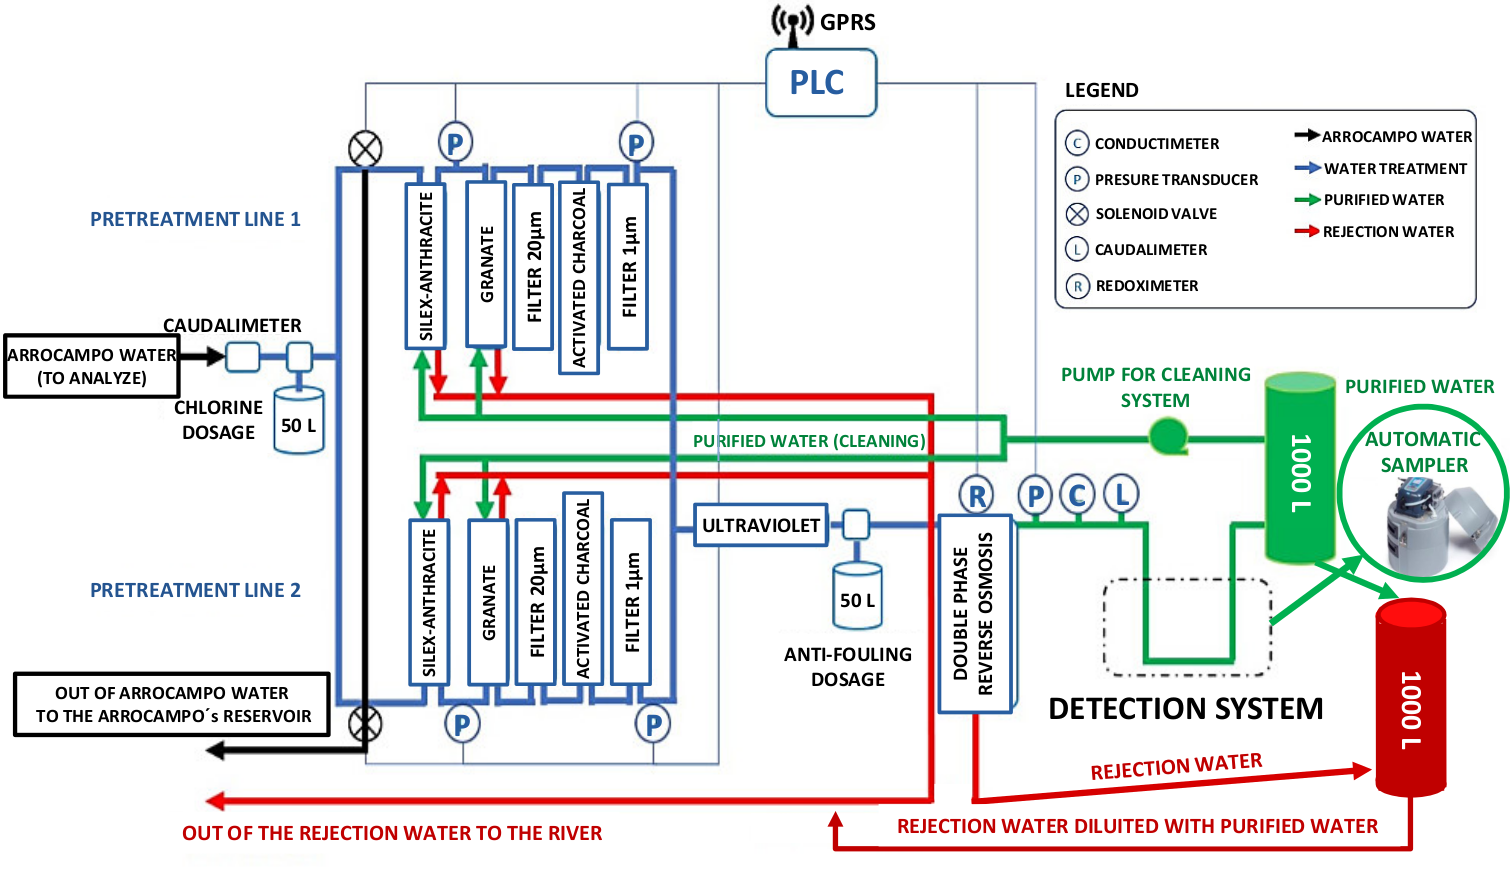
\includegraphics[scale=0.25]{3DesignPrinciples/33UltraPureWaterSystem/SchemeUltraPureWaterSystem.png}
\caption{Scheme of water purification system of TRITIUM.\label{fig:WPSScheme}}
\end{figure}

This system is installed in the Arrocampo dam and consists of four different stages:

\begin{enumerate}
\item{} The raw water from the Tagus river passes through two different filters, the first made of silex-anthracite and the second of garnet, with which a rough filtering is made (the largest particles are eliminated). This system has two identical parallel lines and implements a self-cleaning functions which consist of injecting purified water in the opposite direction.

\item{} The outlet water sample of the first stage, called fine filtration stage, passes through a $20~\mu\meter$ filter (formed by a synthetic mesh) and activated charcoal filters (one per line) that removes chlorine and iron particles present in the water sample.

\item{} The outlet water of the second stage passes through a super-fine filtering consisting of a $1~\mu\meter$ filter, formed of a dense polypropylene mesh and UV lamps. The filter removes all the particles up to diameters of $1~\mu\meter$ and UV lamps sterilize water, eliminating bacteria and microscopic life.

\item{} Finally, the water is introduced in the last stage, double-phase reverse osmosis, that reduces the conductivity of the water to about $10~\mu$S$/\cm$ with only one module of reverse osmosis, enough for the needed conditions. 

\end{enumerate}

As a result of the purification process, besides the pure water that is introduced into the TRITIUM detector, a rejection water is produced,  which contains the particles extracted from the pure water that results in conductivities greater than the original water.

The water purification system is able to process up to $0.850~\meter^3/\hour$ with a single line operating or $1.480~\meter^3/\hour$ with both, greatly outperforming the requirements of the tritium detector. 

The software used for remote controlling the water purification system is Siemens Programmable Logic Controller (Siemens PLC), that gives information such as the state of the valves, the reading of pressure probes and the amount of water production in real time. 

The appendix \ref{App:UltraPureWaterSystem} contains several pictures of different parts of this system, installed in Arrocampo dam.